\documentclass{article}

\usepackage{amsmath,amssymb}
\usepackage{tikz}
\usepackage{pgfplots}
\usepackage{xcolor}
\usepackage[left=2.1cm,right=3.1cm,bottom=3cm,footskip=0.75cm,headsep=0.5cm]{geometry}
\usepackage{enumerate}
\usepackage{enumitem}
\usepackage{marvosym}
\usepackage{tabularx}
\usepackage{multirow}

\usepackage{listings}
\definecolor{lightlightgray}{rgb}{0.95,0.95,0.95}
\definecolor{lila}{rgb}{0.8,0,0.8}
\definecolor{mygray}{rgb}{0.5,0.5,0.5}
\definecolor{mygreen}{rgb}{0,0.8,0.26}
\lstdefinestyle{java} {language=java}
\lstset{language=java,
	basicstyle=\ttfamily,
	keywordstyle=\color{lila},
	commentstyle=\color{lightgray},
	stringstyle=\color{mygreen}\ttfamily,
	backgroundcolor=\color{white},
	showstringspaces=false,
	numbers=left,
	numbersep=10pt,
	numberstyle=\color{mygray}\ttfamily,
	identifierstyle=\color{blue},
	xleftmargin=.1\textwidth, 
	%xrightmargin=.1\textwidth,
	escapechar=§,
}

\usepackage[utf8]{inputenc}
\usepackage{hyperref}
\hypersetup{
	colorlinks,
	citecolor=blue,
	filecolor=blue,
	linkcolor=blue,
	urlcolor=blue
}

\renewcommand*{\arraystretch}{1.4}

\newcolumntype{L}[1]{>{\raggedright\arraybackslash}p{#1}}
\newcolumntype{R}[1]{>{\raggedleft\arraybackslash}p{#1}}
\newcolumntype{C}[1]{>{\centering\let\newline\\\arraybackslash\hspace{0pt}}m{#1}}

\newcommand{\E}{\mathbb{E}}
\DeclareMathOperator{\rk}{rk}
\DeclareMathOperator{\Var}{Var}
\DeclareMathOperator{\Cov}{Cov}
\DeclareMathOperator{\Cor}{Cor}
\DeclareMathOperator{\SD}{SD}

\title{\textbf{Grundlagen des Finanzmanagements, Tutorium 4}}
\author{\textsc{Henry Haustein}}
\date{}

\begin{document}
	\maketitle
	
	\section*{Aufgabe 1: Portfoliotheorie}
	\begin{enumerate}[label=(\alph*)]
		\item Aus der Korrelation sollten wir zuerst die Kovarianz ausrechnen:
		\begin{align}
			\Cor(A,B) &= \frac{\Cov(A,B)}{\SD(A)\cdot \SD(B)} \notag \\
			\Cov(A,B) &= \Cor(A,B) \cdot SD(A)\cdot \SD(B) \notag \\
			&= 0.5\cdot 0.1\cdot 0.1 \notag \\
			&= \frac{1}{100} \notag
		\end{align}
		Damit lassen sich Erwartungswert und Varianz/Standardabweichung der Rendite bestimmen:
		\begin{align}
			\E(r) &= 0.4\cdot 15\text{ \%} + 0.6\cdot 25\text{ \%} = 21\text{ \%} \notag \\
			\Var(r) &= 0.4^2\cdot 0.1^2 + 0.6^2\cdot 0.2^2 + 2\cdot 0.4\cdot 0.6\cdot \frac{1}{100} = 0.0208 \notag \\
			\SD(r) &= \sqrt{0.0208} = 14.42\text{ \%} \notag
		\end{align}
		\item Jetzt ist $\Cov(A,B)=-\frac{1}{100}$ und mit Rechnung wie in (a) folgt $\Var(r)=0.0112$ und somit $\SD(r)=10.58$ \%.
		\item Wenn die Korrelation steigt, so steigt auch die Standardabweichung.
	\end{enumerate}
	
	\section*{Aufgabe 2: Portfoliotheorie}
	\begin{enumerate}[label=(\alph*)]
		\item Es gilt:
		\begin{align}
			\E(R_H) &= 0.25\cdot (-2\text{ \%}) + 0.6\cdot 9.2\text{ \%} + 0.15\cdot 15.4\text{ \%} = 7.33\text{ \%} \notag \\
			\E(R_S) &= 0.25\cdot 5\text{ \%} + 0.6\cdot 6.2\text{ \%} + 0.15\cdot 7.4\text{ \%} = 6.08\text{ \%} \notag
		\end{align}
		\item Es gilt
		\begin{align}
			\Var(R_H) &= 0.25(-2\text{ \%} - 7.33\text{ \%})^2 + 0.6(9.2\text{ \%} - 7.33\text{ \%})^2 + 0.15(15.4\text{ \%} - 7.33\text{ \%})^2 = 33.6291 \notag \\
			\SD(R_H) &= \sqrt{33.6291} = 5.799\text{ \%} \notag \\
			\Var(R_S) &= 0.25(5\text{ \%} - 6.08\text{ \%})^2 + 0.6(6.2\text{ \%} - 6.08\text{ \%})^2 + 0.15(7.4\text{ \%} - 6.08\text{ \%})^2 = 0.5616 \notag \\
			\SD(R_S) &= \sqrt{0.5616} = 0.7494\text{ \%} \notag
		\end{align}
		\item Es gilt
		\begin{align}
			\Cov(R_H,R_S) &= 0.25(-2\text{ \%} - 7.33\text{ \%})(5\text{ \%} - 6.08\text{ \%}) +  0.6(9.2\text{ \%} - 7.33\text{ \%})(6.2\text{ \%} - 6.08\text{ \%}) \notag \\
			& + 0.15(15.4\text{ \%} - 7.33\text{ \%})(7.4\text{ \%} - 6.08\text{ \%}) \notag \\
			&= 4.2516\text{ \%}^2 \notag \\
			\Cor(R_H,R_S) &= \frac{4.2516\text{ \%}^2}{5.799\text{ \%}\cdot 0.7494\text{ \%}} \notag \\
			&= 0.9783 \notag
		\end{align}
	\end{enumerate}
	
	\section*{Aufgabe 10.1: Übliche Maße für Risiko \& Ertrag}
	\begin{enumerate}[label=(\alph*)]
		\item Es gilt
		\begin{align}
			\E(r) = 0.4\cdot (-100\text{ \%}) +  0.2\cdot (-75\text{ \%}) +  0.2\cdot (-50\text{ \%}) +  0.1\cdot (-25\text{ \%}) +  0.1\cdot 1000\text{ \%} = 32.5\text{ \%} \notag
		\end{align}
		\item Es gilt
		\begin{align}
			\Var(r) &=  0.4\cdot (-100\text{ \%} - 32.5\text{ \%}) +  0.2\cdot (-75\text{ \%} - 32.5\text{ \%}) +  0.2\cdot (-50\text{ \%} - 32.5\text{ \%}) \notag \\
			& +  0.1\cdot (-25\text{ \%} - 32.5\text{ \%}) +  0.1\cdot (1000\text{ \%} - 32.5\text{ \%}) = 104631.25 \notag \\
			\SD(r) &= \sqrt{104631.25} = 323.4675\text{ \%} \notag
		\end{align}
	\end{enumerate}

	\section*{Aufgabe 10.12: Diversifikation von Aktienportfolios}
	\begin{enumerate}[label=(\alph*)]
		\item Der Markt hat eine erwartete Rendite von 10 \%. Investiert man nach Methode (i), so kann man nach 2 Jahren $\E(r_{(i)}) = 1.05\cdot 1.1= 1.155 \Rightarrow 15.5$ \% erwarten. Für Methode (ii) gilt $\E(r_{(ii)}) = 1.1\cdot 1.1= 1.21 \Rightarrow 21$ \%.
		\item Folgt man Strategie (i), so kann der Markt im 2. Jahr entweder fallen oder steigen:
		\begin{center}
			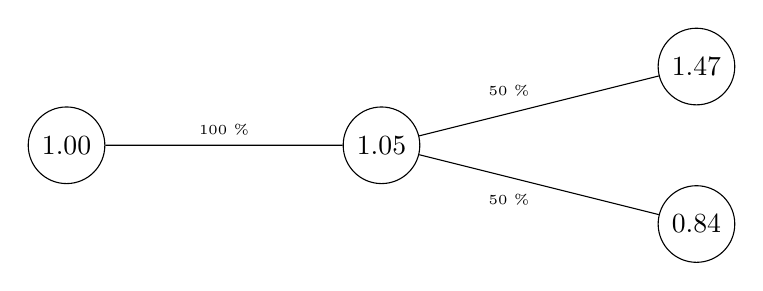
\begin{tikzpicture}
			\node[circle,draw=black, fill=white] (1) at (0,0) {1.00};
			\node[circle,draw=black, fill=white] (105) at (4,0) {1.05};
			\node[circle,draw=black, fill=white] (084) at (8,-1) {0.84};
			\node[circle,draw=black, fill=white] (147) at (8,1) {1.47};
			
			\draw (1) to node[above] {\tiny 100 \%} (105) to node[above left] {\tiny 50 \%} (147);
			\draw (105) to node[below left] {\tiny 50 \%} (084);
			\end{tikzpicture}
		\end{center}
		Die Standardabweichung ist damit 
		\begin{align}
			\SD(r_{(i)}) = \sqrt{0.5(1.47-1.155)^2 + 0.5(0.84-1.155)^2} = 0.315 \notag
		\end{align}
		Bei der Strategie (ii) kann der Markt in beiden Jahren steigen oder fallen:
		\begin{center}
			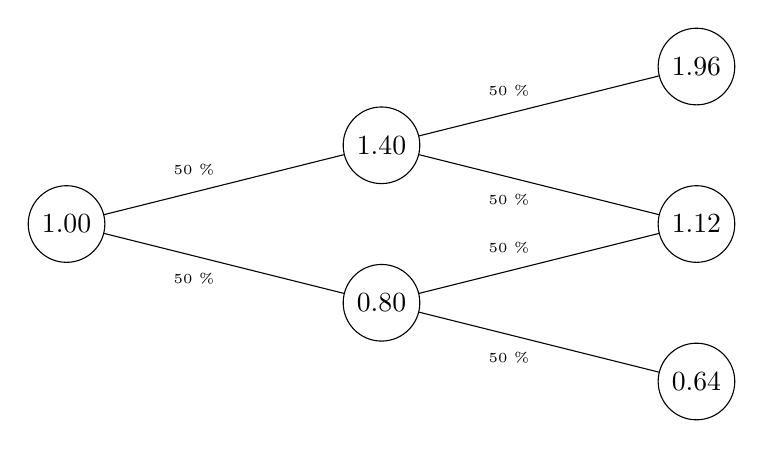
\begin{tikzpicture}
			\node[circle,draw=black, fill=white] (100) at (0,0) {1.00};
			\node[circle,draw=black, fill=white] (080) at (4,-1) {0.80};
			\node[circle,draw=black, fill=white] (140) at (4,1) {1.40};
			\node[circle,draw=black, fill=white] (064) at (8,-2) {0.64};
			\node[circle,draw=black, fill=white] (112) at (8,0) {1.12};
			\node[circle,draw=black, fill=white] (196) at (8,2) {1.96};
			
			\draw (100) to node[above left] {\tiny 50 \%} (140) to node[above left] {\tiny 50 \%} (196);
			\draw (100) to node[below left] {\tiny 50 \%} (080) to node[below left] {\tiny 50 \%} (064);
			\draw (140) to node[below left] {\tiny 50 \%} (112);
			\draw (080) to node[above left] {\tiny 50 \%} (112);
			\end{tikzpicture}
		\end{center}
		Die Standardabweichung ist damit 
		\begin{align}
			\SD(r_{(ii)}) = \sqrt{0.25(1.96-1.21)^2 + 0.5(1.12-1.21)^2 + 0.25(0.64-1.21)^2} = 0.4753 \notag
		\end{align}
		\item nein, es steigt
	\end{enumerate}

	\section*{Aufgabe 10.17: Das Beta und die Kapitalkosten}
	\begin{enumerate}[label=(\alph*)]
		\item Es gilt
		\begin{align}
			r = r_f + \beta\cdot\text{Marktrisikoprämie} = 4\text{ \%} + 1.04\cdot 5\text{ \%} = 9.2\text{ \%}\notag
		\end{align}
		\item Es gilt
		\begin{align}
			r = r_f + \beta\cdot\text{Marktrisikoprämie} = 4\text{ \%} + 0.19\cdot 5\text{ \%} = 4.55\text{ \%}\notag
		\end{align}
		\item Es gilt
		\begin{align}
			r = r_f + \beta\cdot\text{Marktrisikoprämie} = 4\text{ \%} + 2.31\cdot 5\text{ \%} = 15.5\text{ \%}\notag
		\end{align}
	\end{enumerate}
	
	\section*{Aufgabe 10.18: Das Beta und die Kapitalkosten}
	Die Aktie von Autodesk hat zwar eine höhere Rendite, aber auch das Risiko ist größer und damit ist für besonders risikoaverse Investoren wie z.B. Rentenkassen, die Aktie von Autodesk nicht geeignet.
	
\end{document}